\documentclass[12pt,UTF8]{ctexart}
\usepackage{titling,setspace}
\usepackage{enumerate,enumitem}
\usepackage{amsmath,amssymb,amsfonts}
\usepackage{listings}
\usepackage{comment}
\usepackage{float}
\usepackage{graphicx}
\usepackage{multicol,multirow}
\usepackage[unicode=true,%本行非常重要 支持中文目录hyperref CJKbookmarks对二级目录没用
	colorlinks,
	linkcolor=black,
	anchorcolor=black,
	citecolor=black,
	CJKbookmarks=false]{hyperref}
\usepackage{xcolor}
\usepackage{geometry}
\geometry{top=25mm,bottom=25mm,left=25mm,right=25mm}
\pagestyle{plain}%删除页眉
\CTEXsetup[format={\large\bfseries}]{section}
\renewcommand\maketitlehooka{\null\mbox{}\vfill} % 标题页
\renewcommand\maketitlehookd{\vfill\null}

\lstset{language=c++,basicstyle=\tiny,escapechar=`,showstringspaces=false}
\setlength{\droptitle}{-100pt}%减少标题与页眉距离

\setenumerate[1]{itemsep=0pt,partopsep=0pt,parsep=\parskip,topsep=5pt}
\setitemize[1]{itemsep=0pt,partopsep=0pt,parsep=\parskip,topsep=5pt}

\title{{\Huge Project 3\\家谱管理}}

\vspace{100pt}
\author{\vspace{200pt}\quad\\
计科一班 17341009 曾天宇\\
计科一班 17341015 陈鸿峥\\
计科二班 17341059 黄杨峻}
\date{}

\begin{document}
\begin{spacing}{1.4}

\clearpage\maketitle
\thispagestyle{empty}

\newpage
\setcounter{page}{1}
\section{题目要求}
	本次project要求用树形结构实现家族成员信息管理,如建立、删除、查询、统计、打印等。
	我们经过讨论,实现了以下六个功能:
	\begin{itemize}
		\item 实现树的输入与生成,录入家族成员的姓名、性别、出生年份、目前年龄(或享年)、以及家庭关系信息,输入采用\verb'dot'格式输入\footnote{文本图形描述语言dot,\url{https://en.wikipedia.org/wiki/DOT_(graph_description_language)}},形如:
\begin{center}
\begin{lstlisting}
digraph genealogy{
	HYJ [gender="M", birth="1978", age="40"];
	CHZ [gender="M", birth="1999", age="19"];
	ZTY [gender="M", birth="1998", age="20"];
	WIFE [gender="F", birth="2000", age="18"];
	HYJ -> WIFE [label="mate"];
	HYJ -> CHZ [label="kid"];
	HYJ -> ZTY [label="kid"];
}
\end{lstlisting}
\end{center}
		\item 实现树的节点增删,通过人名来检索需要增删的目标。
		\item 实现树节点的查询,并打印节点,使用人名搜索,若查无此人,输出\verb'error message'
		\item 实现树的统计,输出总人数、总代数信息。
		\item 实现树的打印,输出一张csv表格,并用opml的方式在workflowy上可视化展示。
	\end{itemize}

\section{数据结构与算法}
	我们首先定义了\verb'Person'类,用于记录每一个家庭成员的信息,并设置了各类信息的\verb'get'、\verb'set'函数(如\verb'getName'、\verb'setAge'等)。然后我们定义了\verb'Family'类,供家族系统增删查改信息。我们还定义了一个\verb'map<string,Person*>'类型的映射,将每一个家族成员的姓名映射到节点,方便查询,以下详细说明程序的实现方法。

\subsection{数据结构实现}
	在本实验中,我们采用了如下的数据结构:
	\begin{itemize}
		\item \verb'Person'类:对单一个人进行储存,存储内容为:姓名、出生年份、年龄、性别、配偶(可选)、父亲姓名、孩子指针列表。整个结构数据默认初始化为:
		\begin{center}\verb'"" - 1990 - 0 - Male - nullptr - "" - null vector'\end{center}
		\item \verb'Family'类:对家谱进行整体存储。这里不仅用了树形的数据结构,还使用标准库中的\verb'map'对索引进行加速。
	\end{itemize}

	在实现方法上,我们为\verb'Person'和\verb'Family'类设计了尽可能详细的访问函数,将尽可能多的代码简并。特别的是,在插入新的节点的过程中,需要同时对家谱树和索引进行添加;同理删除也是需要这两步操作的。由于前面设计了\verb'map'的数据结构进行辅助,因此在查找的时间复杂度只有$\mathcal{O}(1)$。

\subsection{输入实现}
	在本实验中,我们支持多种输入输出方式。
	考虑到家谱可能十分庞大,故通过一个个结点插入的方式读入显然是不可行的。因此我们采用图形描述语言dot来对家谱进行读入。用于只需按照一定的规则在记事本里定义好家族各个成员之间的联系,并将文件存储为dot格式,即可被我们的程序成功读入。

	具体的dot文件撰写分为两个部分,先要声明所有结点(人)的信息,然后对这些结点建立关系。
	\begin{itemize}
		\item 结点:
		\begin{center}\verb'<name> [gender = <M/F>, birth = <year>, age = <age>];'\end{center}
		\item 关系:
		\begin{center}\verb'<name1> -> <name2> [label = <mate/kid>];'\end{center}
	\end{itemize}
	举例来说,我们要建立名为HYJ这个人的信息,已知他是男的,于1978年出生,年龄40,则我们可以键入
	\begin{center}\verb'HYJ [gender="M", birth="1978", age="40"];'\end{center}
	如果他有一个妻子,名为WIFE,2000年出生,年龄20,则我们可以键入
	\begin{center}\verb'WIFE [gender="F", birth="2000", age="18"];'\end{center}
	同时添加关系
	\begin{center}\verb'HYJ -> WIFE [label = "mate"]'\end{center}
	注意:为了防止有些人早逝导致信息有误,我们还是强制用户输入每个人的年龄。

	具体实施采用以下两条正则表达式对输入字符串进行处理
	\begin{center}\verb'*\[ *gender *= *" *|" *\];| +|", *birth *= *"|", age *= *"'\\
	\verb' *\[ *label *= *"|" *\];| *-> *| +'\end{center}

\subsection{输出实现}
	\begin{enumerate}
		\item xml格式\footnote{可扩展标记语言xml,\url{https://en.wikipedia.org/wiki/XML}}输出\\
		由于xml本身就具有树的性质,故我们可以利用xml格式进行输出,通过输出结点的层次结构可直观看到家谱的形状。例子如下。
\begin{lstlisting}
<family_tree>
    <node>
        <name>HYJ</name>
        <birth>1978</birth>
        <age>20</age>
        <kids>
            <node>
                <name>CHZ</name>
                <birth>1999</birth>
            </node>
        </kids>
        <mate>WIFE</mate>
    </node>
</family_tree>
\end{lstlisting}
		\item csv表格\footnote{逗号分隔符csv,\url{https://en.wikipedia.org/wiki/Comma-separated_values}}输出\\
		利用csv格式输出也是十分直观的方式,将每个人的信息一一罗列在同一行上,输出文件用Excel表即可打开(该方法借鉴了银行流水报告的输出)
		\item workflowy\footnote{Workflowy,\url{https://workflowy.com/}}可视化\\
		我们对前面的xml文件进一步升级,得到opml格式文件\footnote{大纲处理标记语言opml,\url{https://en.wikipedia.org/wiki/OPML}},以便输入workflowy进行可视化
	\end{enumerate}

\section{测试数据、结果及分析}
实验测试结果如图\ref{fig:io}至图\ref{fig:visualization}所示。
可以看见,我们的程序正常执行,输出了正确的结果,并且给出了多种直观的可视化方案。
\begin{figure}[htbp]
\centering
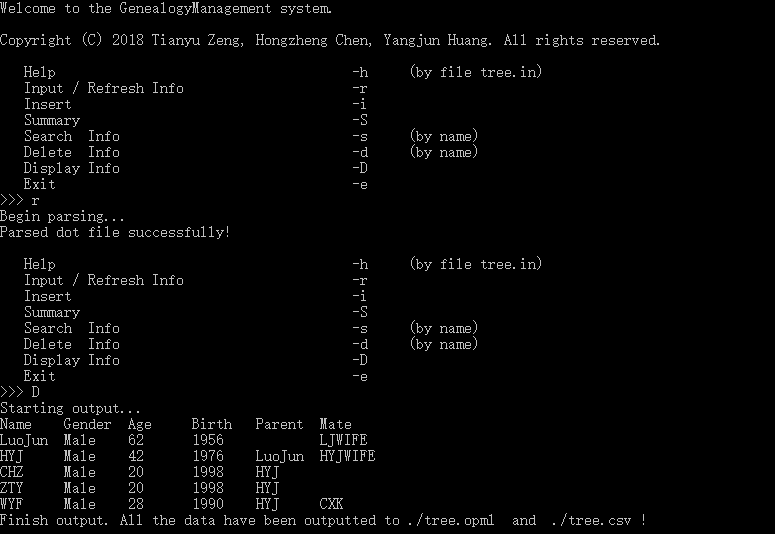
\includegraphics[width=0.9\linewidth]{fig/IO.PNG}
\caption{输入输出(IO)}
\label{fig:io}
\end{figure}
\begin{figure}[htbp]
\centering
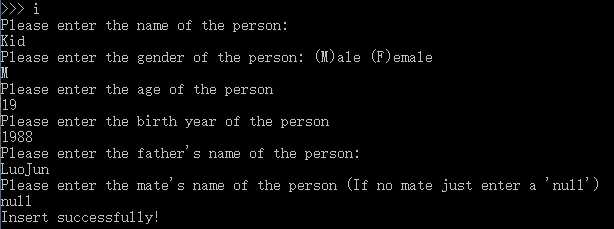
\includegraphics[width=0.6\linewidth]{fig/insert.PNG}
\caption{插入结点}
\label{fig:insert}
\end{figure}
\begin{figure}[htbp]
\centering
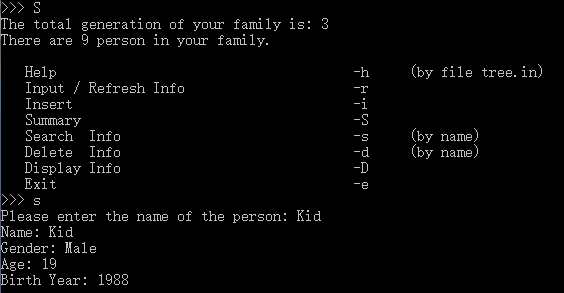
\includegraphics[width=0.6\linewidth]{fig/show_and_search.PNG}
\caption{单一数据查询及多数据展示}
\label{fig:show}
\end{figure}
\begin{figure}[htbp]
\centering
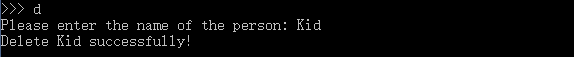
\includegraphics[width=0.6\linewidth]{fig/delete.PNG}
\caption{删除结点}
\label{fig:delete}
\end{figure}
\begin{figure}[htbp]
\centering
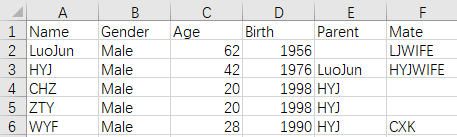
\includegraphics[width=0.8\linewidth]{fig/csv.PNG}
\caption{csv文件输出}
\label{fig:csv}
\end{figure}
\begin{figure}[htbp]
\centering
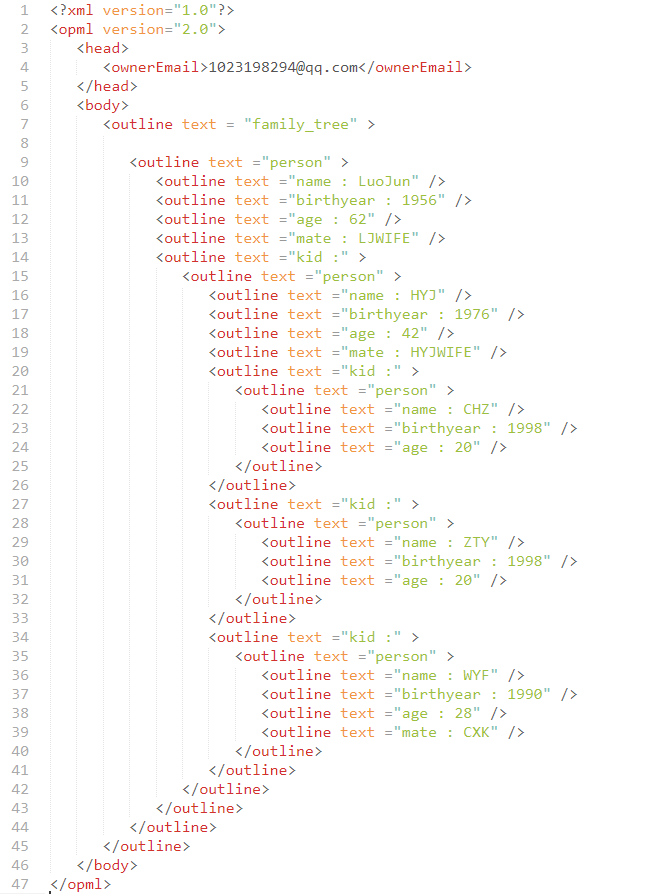
\includegraphics[width=0.8\linewidth]{fig/opml.PNG}
\caption{OPML输出}
\label{fig:opml}
\end{figure}
\begin{figure}[htbp]
\centering
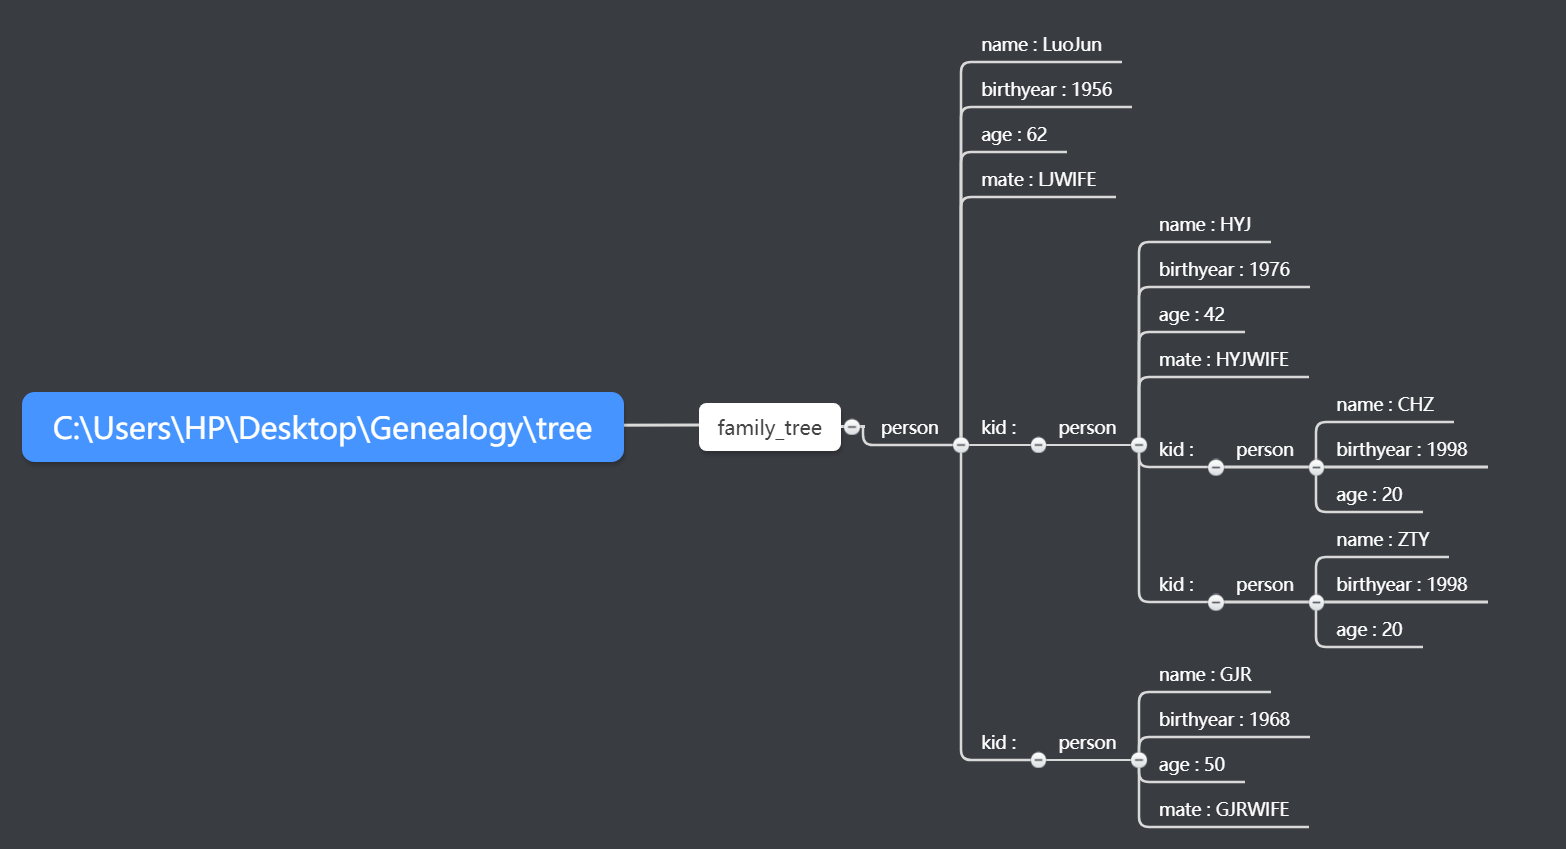
\includegraphics[width=\linewidth]{fig/family_tree.png}
\caption{可视化结果}
\label{fig:visualization}
\end{figure}


\section{分工、贡献与自我评分}
\begin{table}[H]
	\centering
	\begin{tabular}{|c|c|c|c|}
		\hline
		& 分工 & 贡献度 & 自我评分\\
		\hline
		曾天宇 & 实现Person类、Family类,测试修改代码、写实验报告 & 0.33 & 10/10\\
		陈鸿峥 & 实现输入输出功能、测试修改代码、实验报告撰写 & 0.33 & 10/10\\
		黄杨峻 & 实现输入输出界面、生成输出、测试修改代码、写实验报告 & 0.33 & 10/10\\
		\hline
	\end{tabular}
\end{table}

\section{项目总结}
% (收获、体会,若实验课上未完成调试,要认真找出错误并分析原因等。)
这次项目难度不高,涉及到的知识都是树最基础的删改查找,但最困扰我们的问题就是输入输出,我们几乎花了一节课的时间去讨论这个问题,直到最后才删删改改实现了一个大家都比较满意的方案。不过我们这次项目开始之前,先做好了document,规范好了接口,并在个人服务器上建立git仓库,共享代码(图\ref{fig:git}是我们的一些commit的记录),给各自的工作带来不少便利,写代码效率高了不少。
\begin{figure}[htbp]
\centering
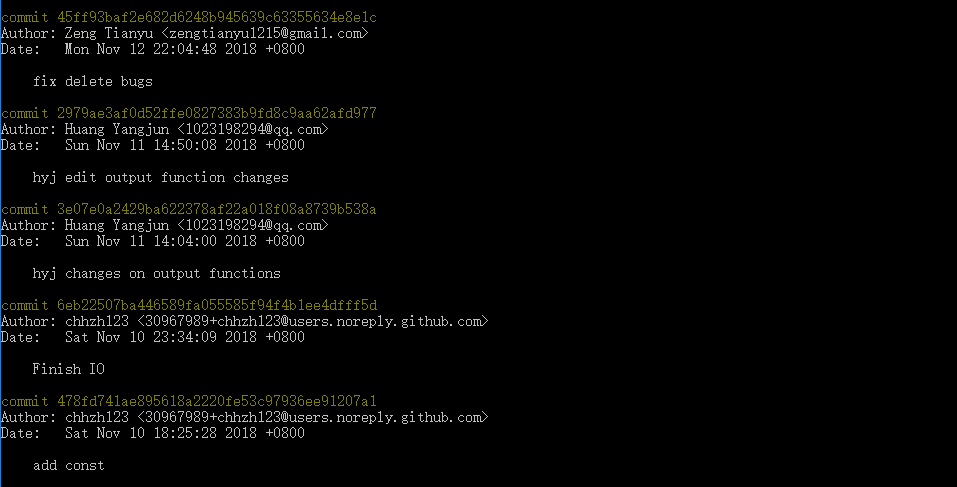
\includegraphics[width=\linewidth]{fig/git.PNG}
\caption{Git commit记录}
\label{fig:git}
\end{figure}

\end{spacing}

%\section{程序清单}
%\subsection{主函数}
%\begin{lstlisting}
%	
%\end{lstlisting}

\end{document}